%%%%%%%%%%%%%%%%%%%%%%%%%%%%%%%%%%%%%%%%%%%%%%%%%%%%%%%%%%%%%%%%%%%%%%
%%% intro.tex
%%% 緒論
%%%%%%%%%%%%%%%%%%%%%%%%%%%%%%%%%%%%%%%%%%%%%%%%%%%%%%%%%%%%%%%%%%%%%%
%%%    「学位論文用TeXフォーマット」
%%%
%%%    岩田 創 --- Takumi IWATA
%%%%%%%%%%%%%%%%%%%%%%%%%%%%%%%%%%%%%%%%%%%%%%%%%%%%%%%%%%%%%%%%%%%%%%
\chapter{緒論}
\label{chap:intro}
%%%%%%%%%%%%%%%%%%%%%%%%%%%%%%%%%%%%%%%%%%%%%%%%%%%%%%%%%%%%%%%%%%%%%%
%%%  main.texから\include : YaTeX用コマンド
%#!platex main.tex
%%%%%%%%%%%%%%%%%%%%%%%%%%%%%%%%%%%%%%%%%%%%%%%%%%%%%%%%%%%%%%%%%%%%%%
\section{天然の流れ星と極超音速環境下での空力加熱}
天然の流れ星は速いもので72~km/sの極超音速で移動し~\cite{williams2004velocity},
流星体が地球大気に突入する際にプラズマ発光を起こす現象である~\cite{nagasawa1997,ceplecha1998meteor,ayers1965luminous,abe2008meteoroids}.
極超音速で飛行する物体前方には強い衝撃波が形成され,
対流加熱により物体は加熱される.
さらに,温度が10,000~K程度になると,原子内の電子が励起され,
脱励起する際に放出される輻射によって物体前方のみならず物体後部も加熱される.
また,この輻射によって我々は天然の流れ星をプラズマ発光現象として目にしている.

流星は自然現象であるため出現時刻・大気突入速度・角度・質量・形状・密度
などの不確定要素が多い.
また,多くの流星体が大気突入の際に焼失するため,その物性を事後調査することも不可能である場合が多い.
そのため,流星の発光の物理現象を正確に解き明かすことは難しいとされている~\cite{ceplecha1998meteor}.

さらに,流星現象への理解が十分になされていない理由として,
高層大気への観測手法の不足が挙げられる.
高層大気観測は現在,全地球に展開しているレーダー・磁気計・光学観測装置・太陽望遠鏡などを用いた高層大気の地上観測ネットワークにおいて行われている.
レーダーにより観測した電波と,カナダやアイスランドなどの極地においてオーロラやそれに伴う現象をカメラで捉えた光を組み合わせて高層大気の諸現象を観測することが現在の主な観測手法である.
また,人工衛星をはじめとする宇宙物体の軌道運動の変化を観測し,
大気状態を推定する方法もある.
2000年に打ち上げられた,高精度の加速度計を搭載した人工衛星CHAMP~\cite{stolle2006magnetic}(図~\ref{fig:champ})は,
熱圏大気質量密度の詳細なデータを10年に渡って計測した.
この観測データは極めて有益なものであり,
高精度加速度計を搭載した衛星による観測が有効であることが示された~\cite{fujiwara2013uchu}.
しかし,これらによる観測が可能なのは,
大気球の場合高度30~km以下,
人工衛星の場合高度300~km以上の範囲に限られている.
大気球や人工衛星の観測領域に入らない高度30~kmから300~kmでは,
観測ロケットによる観測が行われている.
観測実験は多岐に渡って行われてきたが,
観測ロケットを高頻度に打ち上げることは難しいことから観測は1--2~年に1度の頻度であるうえに,
1回の観測時間は数分から数十分と極めて短いため,
継続的かつ中長期的な観測を行うことはできていない.
したがって,高層大気については未だ謎が多いままであり,
特に中間圏という大気区分に属する高度80~kmから200~kmにおける観測データは少ない~\cite{sato2017frequency}.
この領域の大気を観測するためには,
宇宙機や隕石,流星などの大気圏突入物体の軌道解析が有効かつほとんど唯一の手法となる.
しかし,地上に到達する宇宙機や隕石の再突入は稀であり,
その観測機会は十分ではない.
天然の流星や火球の観測はビデオカメラやレーダーを用いて長期に渡り行われているが,
これらは発生時刻や場所の正確な予測が困難であるため,
これらの観測を通して高精度なデータが求まることは稀である~\cite{kimura2018master}.

\begin{figure}[H]
    \centering
    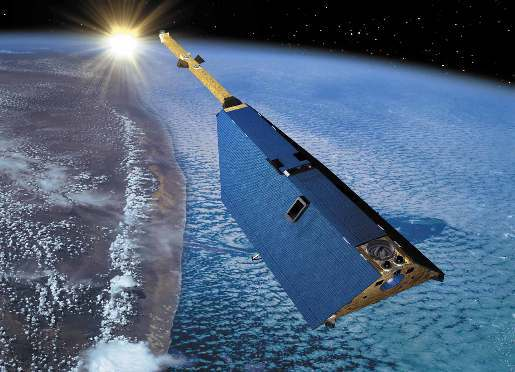
\includegraphics[width=10cm]{fig/intro/CHAMP.png}
    \caption{人工衛星CHAMP~\cite{zehentner2017phd}.}
    \label{fig:champ}
\end{figure}

\section{人工流れ星}

人工流星とは,観測ロケットや宇宙機から流星のもと(以降,流星源)を任意の軌道に投入し,
大気圏に再突入させるなどの方法で人工的に発生させる流星のことである.
形状や密度などの条件が既知な流星源を適切な軌道に投入して大気圏へ再突入させれば,
流星の発生時刻や場所が予測できるため,
高精度の科学観測を実施することが可能である.
また,観測ロケットや宇宙機からの放出速度・放出角度を制御することで,
任意の地点で人工流星を発生させることも可能となり,
観測場所への制約なく観測を行うことができる.

人工的に流星を発生させる構想は古く,1940年代からあるとされる.
世界初の人工流星実験は1946年にFritz ZwickyらによってドイツV2ロケットを用いて実施されているが,
ロケットの爆発により失敗に終わった.
1957年には同じくV2ロケットを用いて米国空軍がホワイト・サンズで実験を行い,
数~cmのアルミニウム球が3発埋め込まれた釣鐘型弾薬を高度87~kmで爆発させることで15~km/s程度まで加速させ,
人工流星を発生させることに成功している.
その後,1960~年代には,
NASAのラングレー研究所によって天然流星のパラメータを決定する目的での人工流星実験が複数回行われている.
この実験では,観測ロケットで飛行中に数~cmほどの金属プロジェクタイルを約12~km/sで大気圏突入させ,
0等級ほどの人工流星を10個発生させた.
この人工流星の発光はスーパーシュミットカメラなど4種類のビデオカメラによって観測され,
低速の流星について,流星発光モデルの計算で用いる発光効率が高精度で求まるなどの成果があった.
1970年以降は観測ロケットを用いた人工流星実験は行われていないが,
さらなる人工流星実験を待ち望む研究者も存在する.

地球に再突入する宇宙機も人工流星と同様に観測に活用されたことがあり,
Genesisカプセル,Stardustカプセルのほか,小惑星サンプルリターン探査機「はやぶさ」がその例として挙げられる.
はやぶさは2010年に地球に帰還したが,
その際にはカプセルのみならず探査機本体も惑星間空間から地球大気圏に約12~km/sの速度で再突入し,
明るく輝く人工火球となった(図~\ref{fig:hayabusa}).
その再突入観測では,
流星の物理モデルにおける摩耗係数や発光効率が算出されるなどの成果が挙げられ,
貴重な観測例となっている.
それ以外にも分光観測や,流星が形成する衝撃波とそれが発生させる超低周波音である衝撃波・インフラサウンド観測が行われた.
このように,人工流星は不明なパラメータの多い天然流星のデータ較正に役立つほか,
大気の密度や組成,上空での空気の流れを知るための発光観測にも貢献することができ,
大きな科学的意義がある.

現在,Astro Live Experience社(以降,ALE)~\cite{ALECoLtd30:online}は,人工流れ星プロジェクトに取り組んでいる.
当該プロジェクトは,直径1~cm程度の流星源を人工衛星に複数搭載して進行方向後ろ向きに放出し,
大気圏に再突入させることで流星現象を人工的に模擬する試みである.
人工衛星を用いた人工流星は観測ロケットを用いた人工流星と比べてコストを抑えることができ,
一度打ち上げを行った後は搭載した流星源が尽きるまでミッションを継続することができる.
ALE人工流星は,天然流星よりも明るく大気の電離も顕著であるため,有効な観測手法になる.
また,人工流星は発光時間・場所を事前に認知でき,天然流星では高度的に観測が困難であった中間圏周辺を観測できるようになることが期待される~\cite{hiraga2017ale}.

ALE人工流星は素材や成分組成等の物性が既知であり,
その発光を観測し天然流星の発光現象と比較することで,
天然流星の光度曲線や成分組成,熱による変化から流星体の分裂と行った諸現象の理解につながると考えられる~\cite{jenniskens2000meteors}.

\begin{figure}[H]
    \centering
    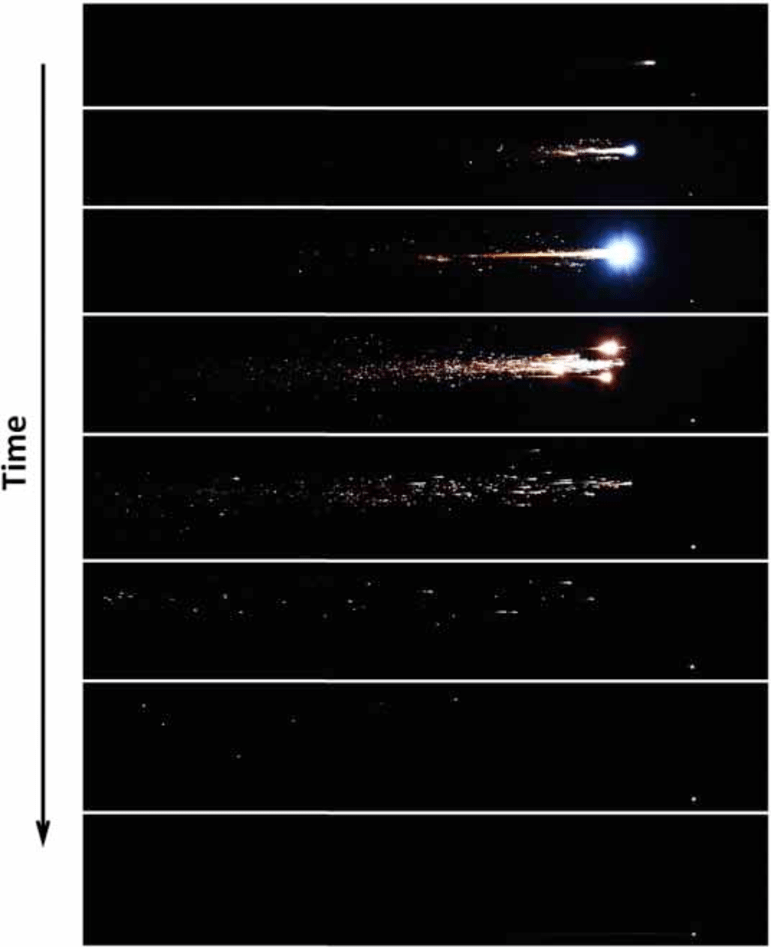
\includegraphics[width=10cm]{fig/intro/hayabusa.png}
    \caption{「はやぶさ」カプセル帰還時の発光の様子~\cite{grinstead2011airborne}.}
    \label{fig:hayabusa}
\end{figure}



\section{人工流れ星周りの流体場解析手法}

人工流れ星は人工衛星が移動する高度から放出され,再突入の過程で焼失する.
放出から焼失の間に流星源は高度を落とし,大気密度は上がっていく.
従って,流星源周りの流体場は自由分子流から希薄流,そして連続流になっていくということが予想される.

連続流の解析にはNavier–Stokes方程式を数値的に解く手法(以降,Navier–Stokes解析)が一般に用いられる.
Navier–Stokes解析では気体分子の粒子群を連続体としてみなしているため,
粒子の性質を表現することが難しい.
粒子が他の粒子と衝突してから,再度他の粒子と衝突するまでの距離の平均値を
平均自由行程といい,
この平均自由行程が代表長さに対して無視できないほど大きい流れを
希薄流体と呼ぶ.
希薄流体では連続体近似が破綻するため,Navier–Stokes解析を行うことが困難になる.
この希薄流体に対する解析手法としてDirect Simulation Monte Carlo法~\cite{bird1994molecular}(以降,DSMC法)がある.
DSMC法は粒子の運動を追跡する直接的な手法であるため,粒子数に比例して計算コストが高くなる.
従って,DSMC法は自由分子流に近いほど計算コストが下がり,連続流に近いほど計算コストが上がる.

\section{本研究の目的}

流星周りの流れ場解析はすでに行われているものの~\cite{silber2017shock},
ALE人工流れ星は観測との比較を行うことができるという利点がある.
従って本研究では,ALE人工流れ星を研究対象として,
\begin{itemize}
    \item 極超音速希薄流体場の特性理解
    \item 流星の発光メカニズムの解明
\end{itemize}
を目的として,流体場の数値解析を行う.

ALE人工流星の流体解析はWatanabeらにより行われているが~\cite{watanabe2016development},
アブレーションによる流星源直径の減少が考慮されていない.
そこで本研究ではまず,流体解析の条件決定のために軌道計算を行う.
すでに木村~\cite{kimura2018master}により軌道計算が行われているが,
正確な定量的議論が行えないことや,流体解析と軌道計算の連成計算も見据えて,
独自に軌道計算シミュレータを構築し,その結果を流体解析の条件として用いる.
次にNavier–Stokes解析およびDSMC法を用いて流体場解析を行い,目的達成を試みる.


\section{本論文の構成}

第\ref{chap:intro}~章では研究背景・先行研究・研究目的について述べた.
第\ref{chap:methods}~章では軌道計算・Navier–Stokes解析・DSMC法における支配方程式や物理モデルなどの解析手法を述べる.
第\ref{chap:trajectory}~章では軌道計算の条件および結果を示し,先行研究との比較を行う.
第\ref{chap:min-knud}~章では希薄流が予想される流星源周りにおいてNavier–Stokes解析とDSMC法の使い分けが必要となるかの調査を目的として,
軌道計算で得られたKnudsen数分布において最小値をとる高度における流体場解析を行う.
第\ref{chap:couple}~章では軌道計算とDSMC法を連成させた解析を行い,DSMC法による補正を加えた高精度な軌道計算を達成する.
第\ref{chap:conclusion}~章では本研究の結論を述べる.



